\section{Planning}%
\label{sec:orga82318d}
In fig.~\ref{fig:gantt-diag2} is illustrated the Gantt diagram for the project
and in fig.~\ref{fig:gantt-tasks} the tasks' descriptions. It should be noted
that the project tasks of Analysis, Design, Implementation and Tests are
performed in two distinct iterations as corresponding to the Waterfall project
methodology.

Due to unpredictable circumstances, limiting the mobility of team
staff and goods, the implementation stage will not be done at full extent, but
rather at a simulation stage. Thus, to overcome these constraints, the project
focus is shifted to the simulation stage, where an extensive framework as to
built to model the system operation, test it, and providing valuable feedback
for the dependents modules. As an example, the modules previously connected just
by an RS232 link, must now include upstream a web module (TCP/IP) --- the data
is now effectively sent through the internet, and must be unpacked and delivery
serially as expected if only the RS232 link was used.

The tasks are described as follows:
\begin{itemize}
\item \uline{Project Kick-off}: in the project kick-off, the group is formed and the tutor
is chosen. A brainstorming about conceivable devices takes place, whose
viability is then assessed, resulting in the product concept definition
(Milestone 0).
\item \uline{State of the Art}: in this stage, the working principle of the device is
studied based on similar products and the system components and its
characteristics are identified.
\item \uline{Analysis}: In the first stage --- Analysis 1 --- contains the analysis
results of the state of the art. It should yield the specifications document,
containing the requisites and restrictions to the project/product, on a
quantifiable basis as required to initiate the design; for example, the
car maximum velocity must be, at maximum, \texttt{2 m/s}. The second stage --- Analysis 2
--- contains the analysis of the first iteration of the development cycle.
\item \uline{Design}: it is done in two segments: modules design --- where the modules are
designed; integration design --- where the interconnections between modules is
designed. It can be subdivided into \emph{conceptual design} and \emph{solution
design}. 
\begin{itemize}
\item In the conceptual design, several problem solutions are identified,
quantifying its relevance for the project through a measuring scale,
inserted into an evaluation matrix, for example, Quality Function Deployment
(QFD).
\item In the solution design, the selected solution is developed. It must include
the solution modelling, e.g.:
\begin{itemize}
\item \uline{Control system design}: analytically and using simulation;
\item \underline{Transducer design}: circuit design and simulation;
\item \underline{Power system design}: power supply, motors actuation and
  respective circuitry design and simulation;
\item \underline{Communications design}: communication protocols evaluation and selection;
\item \underline{Software design}: for all required modules, and considering its
  interconnections, at distinct levels:
  \begin{itemize}
  \item \uline{frontend level}: user interface software, providing a easy and convenient
    way for the user to control and manage the system.
  \item \uline{framework level}: software required to emulate/simulate and test the
    required system behaviour, providing seamless interfaces for the dependents
    modules
  \item \uline{backend level}: software running \emph{behind the scenes}, handling user
    commands received, system monitoring and control.
  \end{itemize}
\end{itemize}
\end{itemize}
\item \uline{Implementation}: product implementation which is done by \uline{modules} and
\uline{integrated}. Once again, it should be noted that the implementation is
mostly done in simulation and coding stages, due to the aforementioned
constraints. In the first stage, the implementation is done in a prototyping
environment --- the assisting framework developed, yielding version alpha; in the second stage
it must include the coding on the final target modules, yielding
prototype beta.
\item \uline{Tests}: unit tests --- \uline{by modules} --- and integrated tests are
performed. Tests are generally considered as those performed over any physical
component or prototype. Here, it is used as a broader term, to reflect the tests
conducted into the system and the several prototypes.
\item \uline{Verification/Validation}: in normal circumstances, after the alpha
  prototype is built the specifications listed in the analysis must be verified
  and the prototype validated by an external agent (an external user to the
  group). Due to abnormal circumstances, the verification must now be performed,
  not on the physical prototype, but over the chain of modules developed,
  checking their performance against the specifications listed, i.e., subsystem
  verification. System verification may be performed to validate overall
  function, but not for quantifiable measurement, due to the latencies
  involved. Regarding validation, once again, there is limited access to the
  physical modules, specially for an external agent, thus, it should be limited
  to user interface validation.
\item \uline{Delivery}: --- project closure encompassing:
\begin{enumerate}
\item Final prototype
\item Support documentation: how to replicate, instruction manual.
\item Final report
\item Public presentation
\end{enumerate}
\end{itemize}

\begin{figure}[!htbp]
\centering
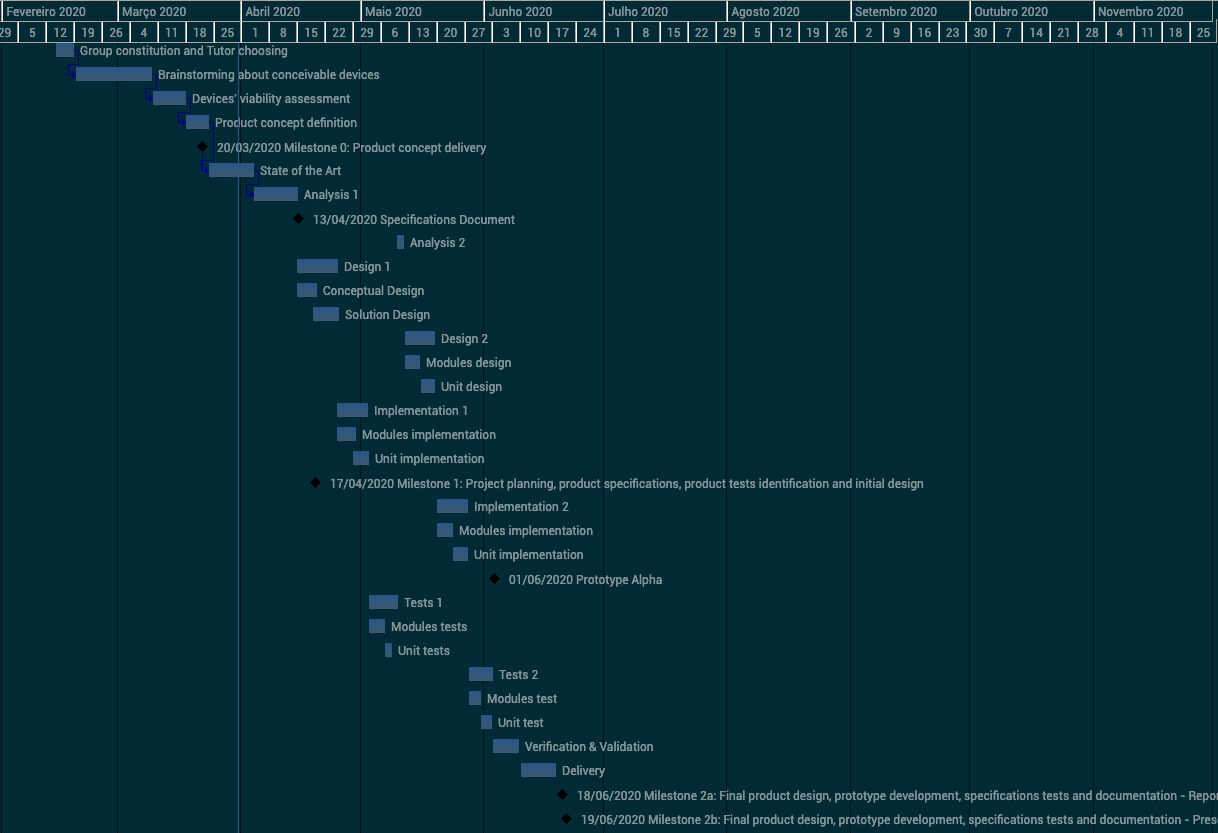
\includegraphics[width=1.0\textwidth]{./sec/img/gantt-diag-orig.png}
\caption{\label{fig:gantt-diag2}Project planning: Gantt diagram 1}
\end{figure}
\begin{figure}[!htbp]
\centering
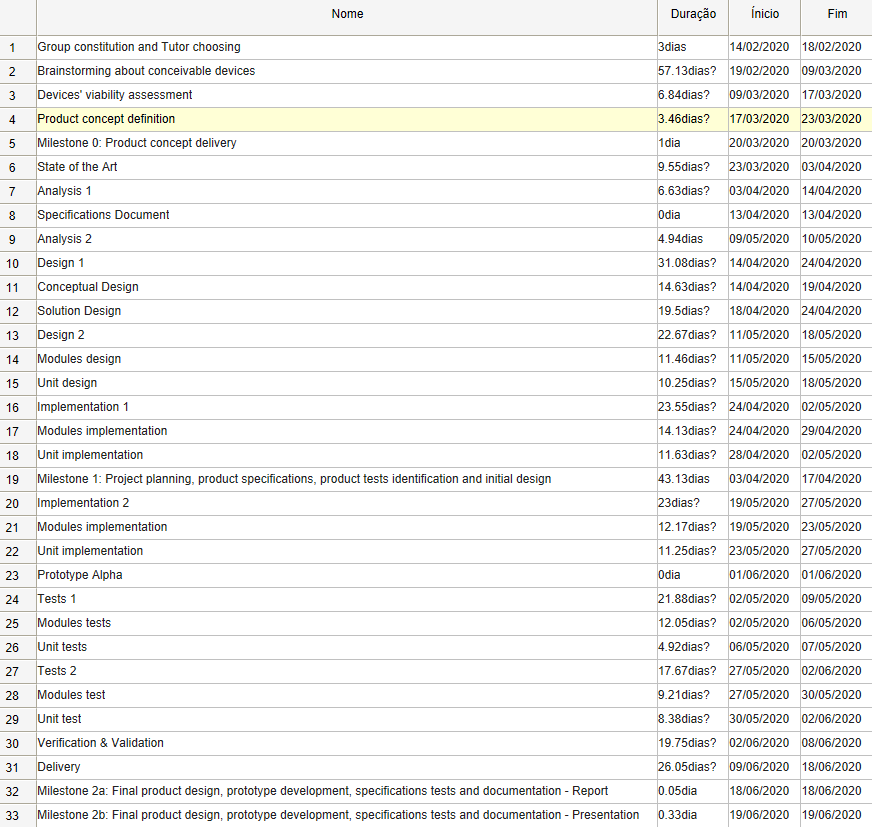
\includegraphics[width=1.0\textwidth]{./sec/img/gantt-orig-tasks.png}
\caption{\label{fig:gantt-tasks}Project planning: tasks}
\end{figure}
%%% Local Variables:
%%% mode: latex
%%% TeX-master: "../Phase1"
%%% End:
